\documentclass[10pt,a4paper]{article}
\usepackage[utf8]{inputenc}
\usepackage{amsmath}
\usepackage{amsfonts}
\usepackage{amssymb}
\usepackage{graphicx}
\usepackage{float}
\usepackage[table, svgnames, dvipsnames]{xcolor}
\usepackage{makecell, cellspace, caption}

\author{Nicolò Brandizzi}
\title{Multi-Agent System Summary}
\date{November 2018}
\begin{document}



\begin{titlepage}
    \begin{center}
        \vspace*{1cm}
        
        \Huge
        \textbf{Multi Agent System Summary}
        
        
        \vspace{1.5cm}
        
        Author:
        \textbf{Nicolò Brandizzi}\\
        \vspace{0.5cm}
        \Large
        Contributors:
        \textbf{}%add contributors here
        
        \vfill
        
        
\includegraphics[width=0.4\textwidth]{images/sapienza_logo.jpg}


        
        \vfill
        
  

        \vspace{0.8cm}
        
        
        \Large
        DIAG\\
        Sapienza\\
        November 2018

    \end{center}
\end{titlepage}


\tableofcontents
\newpage
\begin{abstract}
This is \textbf{free} material! You should not spend money on it.\\
Find the complete material on GitHub \url{https://github.com/nicofirst1/AI_notes}.\\

This notes are about the \textit{Multi Agent System} part taught by professor Daniele Nardi in the Artificial Intelligence class. Everyone is welcome to contribute to this notes in any relevant form, just ask for a pull request and be patient.\\ Remember to add your name under the contributors list in the title page when submitting some changes (if you feel like it).
\end{abstract}



\newpage


\section{Adversarial Games}
\subsection{Games}
In AI a common game has the following proprieties:

\begin{itemize}
\item \textbf{Zero-sum}: is when the total payoff to all player is the same for every instance of the game (better called \textit{constant-sum}) \footnote{An example is chess where you can either win +1, loose -1 or draw 1/2 so that the sum of two player is always 1.}.

\item \textbf{Perfect Information}: everything in the game is visible \footnote{Not like games like poker in which not all the cards are visible.}.

\item Multi-agent with \textit{equal and opposite utility values} \footnote{One player wins the other looses (adversarial).}.

\end{itemize}


Moreover a game is composed of the following elements:
\begin{itemize}
\item Initial state
\item \textit{Players(s)}: which player has to move in a state.
\item \textit{Actions(s)}: return set of legal states.
\item \textit{Result(s,a)}: defines the result of an action (transition-model).
\item \textit{Terminal-Test(s)}: true when the game is over, false otherwise.
\item \textit{Utility(s,p)}: defines the final numeric value for a game that ends in the \textit{terminal state s} for a player $p$.
\end{itemize}

Given the initial player $MAX$ and the other player $MIN$,
we can look at a game as a tree where each node is a state and the edges are moves, by doing so it is easy to get how the player $MAX$ generates an $OR$ node while the player $MIN$ generates an $AND$ node \footnote{Just like in the non-deterministic search problem, we don't know what MIN action will be as we do not know if a non action has occurred in a sensor-less environment.}. This is because MAX do not know which will be the action chosen by MIN so it has to build a \textit{contingent plan} in order to consider every possible outcome.\\

The \textbf{MinMax strategy} is a strategy with the following heuristic:
\[MinMax(s)=\\
\left{
\begin{tabular}{c\quad c}

\begin{cases} Utility(s) & \mbox{if } TerminalTest(s)  \\ 
\max_{a \in Actions(s)}MinMax(Result(s,a)) & \mbox{if } Playes(s)=Max\\
\min_{a \in Actions(s)}MinMax(Result(s,a)) & \mbox{if } Playes(s)=Min\\

 \end{cases}

\end{tabular}
\right}
\]
That is the minmax value of a node is the utility (for MAX) of being in that state, assuming that both players play optimally  \footnote{If MIN is not optimal than MAX will do even better.}.

\paragraph{MinMax Algorithm} It make use of a recursive computation of the minmax values of each successor state, than the values are backed up through the tree as the recursion unwinds. It is like a depth-first exploration where the maximum dept of the tree is $m$ and there are $b$ legal moves.
\begin{itemize}
\item \textbf{Complete}: yes, if $m < \infty$
\item \textbf{Optimal}: yes, if MIN is optimal.
\item \textbf{Time complexity}: $O(b^m)$
\item \textbf{Space complexity}: $O(b\cdot m)$
\end{itemize}

\paragraph{Multiplayer games}
Instead of a value for each node there is a vector, one value for each agent in the game.\\ 
Alliances may arise from purely selfish behavior.

\subsection{Alpha-Beta Pruning}
It is used to prune away branches that cannot influence the final decision. The logic is pretty simple:\\
Consider a node $n$ (in the figure it is the node C) somewhere in the tree, such that MAX can choose to move to that node (since MAX starts form A he can choose between either [B,C,D]). If there is a better choice $m$ at $n$ parent or any point up (in this case the better move would be node B since MIN will chose the minimum value which is 3, if C is considered then MIN could chose $2<3$), then $n$ will never be reached, hence it can be pruned.

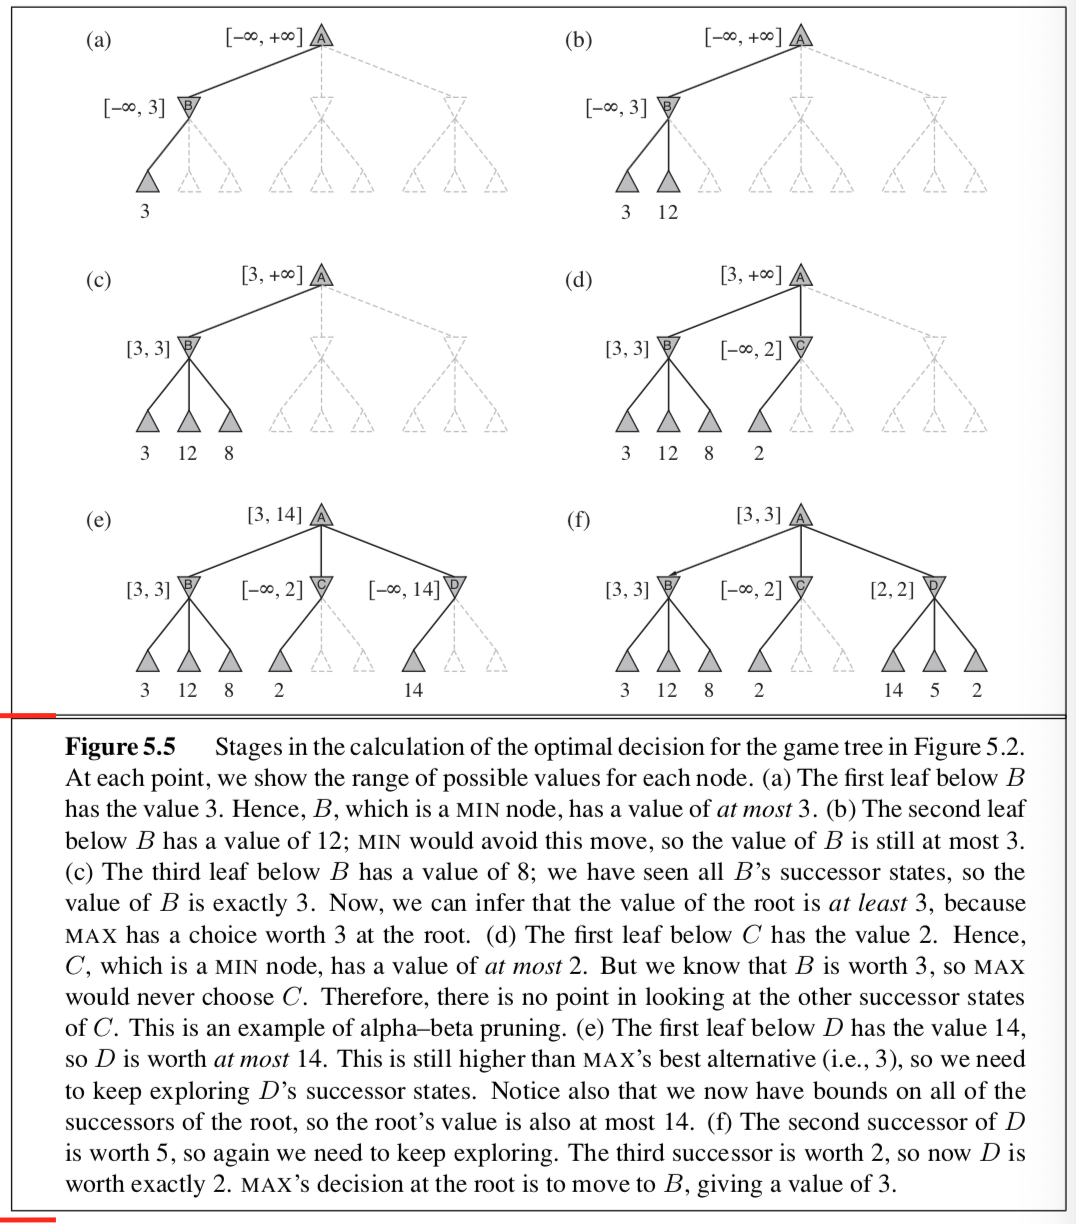
\includegraphics[scale=0.5]{images/alpha_beta_ex.png}

The name alpha-beta derives from the bipolarity of the standard two player game:
\begin{itemize}
\item $\alpha$ is the value of the best choice for MAX, i.e. highest value
\item $\beta$ is the value of the best choice for MIN, i.e. lowest value
\end{itemize}
Each one comes after the other with alpha starting.

\paragraph{Move Ordering} since alpha-beta pruning is dependent on the order in which the states are examined it may be convenient to order them from the lowest to the highest, thus pruning a large part of the search space theoretically bringing the time complexity to $O(b^{m/2})$. On the other hand by examining the successors in a random order we can get a time complexity of $O(b^{3m/4})$.\\
We can use \textbf{dynamic move-ordering schemes}, that first try the moves that were found out to be the best in the past.\\
A \textbf{transposition table} is a way to store the evaluation of the resulting position in a hash table, so that we do not have to recompute it on subsequent occurrence.

\subsection{Imperfect Real-Time Decisions}
We can use an evaluation function as the cutoff value for iterative deepening instead of a fixed depth $d$. This will turn non-terminal nodes into terminal leaves. This can be easily done by slightly modified the minmax algorithm including a heuristic function EVAL which estimates the position utility and replace the terminal test with a \texbf{cutoff test} that decides when to use EVAL.

\paragraph{Evaluation Functions}
How do we design a good evaluation function?
\begin{enumerate}
\item The evaluation function should order the terminal states in the same way as the true utility function ($win> draw> loss$).
\item Computation must not take too long.
\item The evaluation function should be correlated with the actual chances of winning.
\end{enumerate}

How can we get a correlation between estimated and real evaluation functions?\\

We can have features that taken together defines \textit{equivalence classes} of states: the states in each category have the same values for all the features.\\
The evaluation function can return a single value that reflect the proportion of states with each other, for example:\\ 
We know that, in chess, when we encounter the two-pawns vs. one-pawn category there is a 0.72 chance of winning (+1), 0.2 of drawing (0), 0.08 of loosing ($\/2$), so we can use the \textbf{expected value}: 
\[(0.72\cdot 1)+(0.2 \cdot 0)+(0.08 \cdot +1/2)=0.76\]
This kind of evaluation function is called \textbf{weighted linear function} because it can be expressed as:
\[Eval(s)=w_1f_1(s)+w_2+f_2(s)+...+w_nf_n(s)=\sum_{i=1}^nw_if_i(s)\]
where $w_i$ is a weight and $f_i$ is a feature \footnote{There can also be a non linear combination of features.}.

\paragraph{Cutting off search}
We can use incremental depth on each recursive call with iterative deepening, using a \textit{CuttOff-Test(state,depth)} function. When the time runs out the program return the move selected by the deepest complete search.\\
There are some cases in which the approximated nature of the evaluation function has to be addressed, we introduce the notion of \textbf{quiescent} position, which are those position that are unlikely to exhibit wild swings in value in the near future. With this we ca use a \textbf{quiescent search}.\\
Another problem is the one of the \textbf{horizon effect} in which the program is delaying an unavoidable move which will deal serious damage, doing so it can choose some bad moves which will be worst as soon as the unavoidable action takes effect. We can mitigate this behavior using \textbf{singular extension}, a move that is \textit{clearly better} than all other moves in a given position is saved for later search.

\paragraph{Forward pruning}
This technique mimic the human brain that cannot process so many possibilities at once, thus pruning  some moves at a given node immediately without further consideration. Local \textbf{beam search} can be used where the beam is the set of $n$ best moves.\\
We can use the \textbf{ProbCut} function, which is a kind of forward pruning version of alpha-beta search that uses statistic generated from prior experiences.

\subsection{Stochastic Games}
In stochastic games there is a random element which cannot be consider a priori. This leads to the creation of so called \textbf{chance nodes} in addition to AND, OR ones.\\
We use a \textbf{expect-minmax value}, in which for each position we calculate the \textit{expected value} with the average over all possible outcomes. 
\newpage











\section{Communication}
The difference between agents and object oriented programs, is that agents can neither force other agents to perform some action, nor write data onto the internal state of other agents, thus the communication is an \textbf{action} that attempts to influence other agents.

\subsection{Speech Acts}
In \textit{Speech theory}, speech is an action just like any other.

\paragraph{Austin}
Has been the first to study the influence of speech in the environment. He identified a number of \textit{performative verbs} which corresponds to different types of speech acts such as \textit{requests, inform and premise}.

\paragraph{Searle}
Given a SPEAKER who request a HEARER to perform an ACTION, the following proprieties must hold:
\begin{itemize}
\item \textbf{Normal I/O conditions}, where the HEARER is able to hear and the circumstance is normal (not in a movie).
\item \textbf{Preparatory conditions}: HEARER must be able to perform ACTION and SPEAKER believes that HEARER is able to perform ACTION.
\item \textbf{Sincerity conditions}: request must be sincere
\end{itemize}

There is also a division in category for the speech acts:
\begin{itemize}
\item \textbf{Representative}: informing.
\item \textbf{Directives}: requesting (do something).
\item \textbf{Commissives}: promising.
\item \textbf{Expressives}: thanking (express psychological state).
\item \textbf{Declarations} declare war (effect some changes).
\end{itemize}

\paragraph{Plan-based theory for speech acts}
There are two kind of precondition for a speech act (such as the \textit{Request} act):
\begin{itemize}
\item \textit{CanDo} preconditions (cando.pr): The SPEAKER believes that the HEARER is able to do the ACTION
\item \textit{Want} preconditions (want.pr): The SPEAKER must want the action to be performed.
\end{itemize}

The effect of this \textit{Request} action is that the agent will come to believe it wants to do something if it believes that another agent believes it wants to do it. This is also the definition of \textit{CasueToWant}.\\
On the other hand the \textit{Inform} action has to goal for a SPEAKER to get a HEARER to believe some statement; the cando.pr is that the SPEAKER must believe the information $\phi$ and it believes that the hearer must believe that the SPEAKER believe $\phi$.


\subsection{Agent Communication Languages}

\paragraph{KIF}
Stands for \textit{Knowledge Interchange Format} is a communication language for expressing proprieties of a particular domain, i.e. message \textit{content} \footnote{Not messages themselves.}. It it based on first-order-logic and can express the following:
\begin{itemize}
\item properties of things in a domain (e.g. 'Michael is a vegetarian')
\item relationships between things in a domain (e.g. 'Michael and Janine are married')
\item general properties of a domain (e.g. 'everybody has a mother') 
\end{itemize}

The kind of quantifiers it can use are \textit{and, or, not, forall, exists}.

\paragraph{KQML}

Is a message-based language for agent communication where each message has a \textbf{performative} (the class of a message) and some \textbf{parameters}; here is an example:
\textit{
\\(ask-one\\
	:content (PRICE IBM ?price)\\
	: stop-server\\
	:language LPROLOG\\
	s:ontology NYSE-TICKS\\
)\\
}

Where the class is \textit{ask-one}, and each parameter has the following meaning
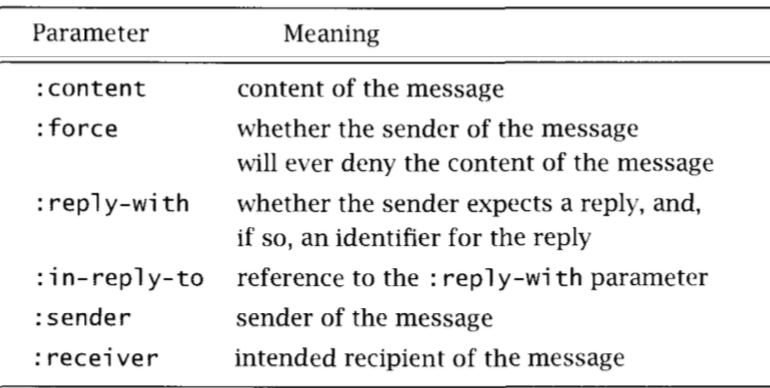
\includegraphics[scale=0.5]{images/KQML_params.png}

\paragraph{FIPA}
Stands for \textit{Foundation for Intelligent Physical Agents} developed a stander for multi-agent communication with \textit{20 performatives} shown below\\
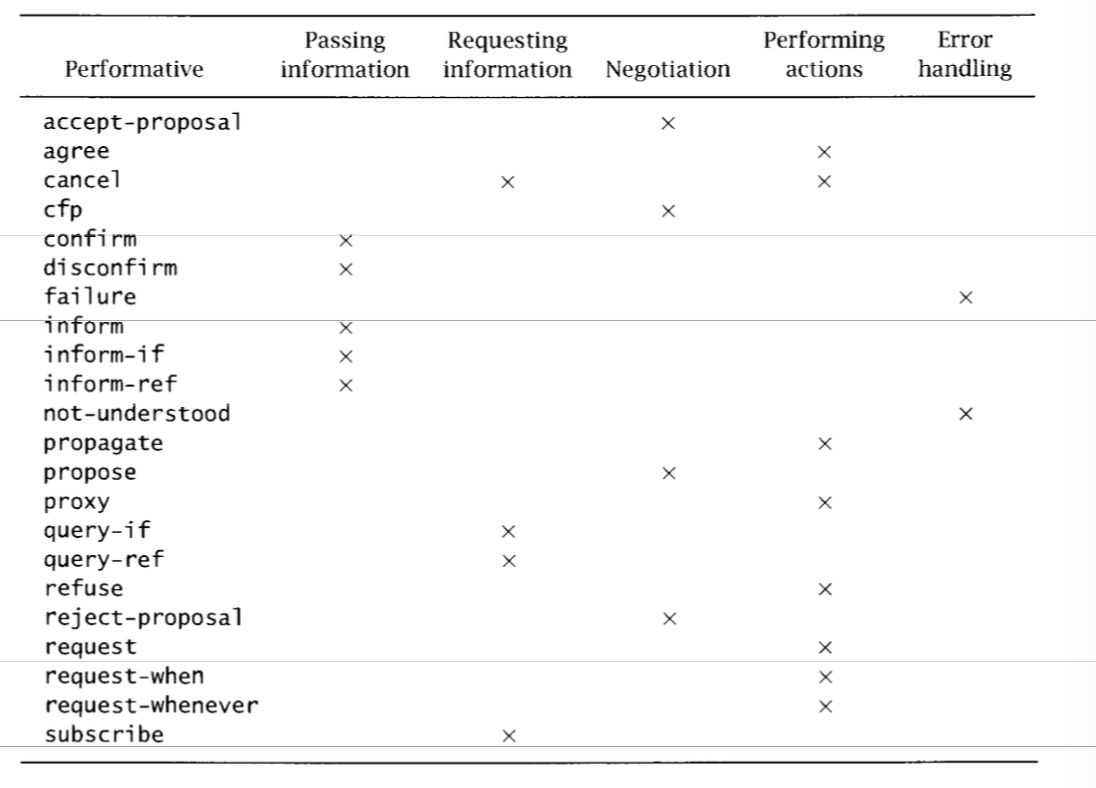
\includegraphics[scale=0.5]{images/KQML_performatives.png}\\

Where :
\begin{itemize}
\item \textit{cfp} is \textit{call for proposal}
\item \textit{inform-if} can be translated with "tell me if the content of the inform-if is either true or false"
\item \textit{inform-ref} same as above but with values
\end{itemize}

The primitives in the FIPA language are:
\begin{itemize}
\item \textit{Inform(i,j,$\phi$)}: where agent $i$ inform agent $j$ about $\phi$. Which have as effect the fact that $j$ now believes $\phi$ ($B_j\phi$) and as preconditions $B_i\phi \wedge \neg B_i(Bif_i\phi \vee Uif_i\phi)$
where:

\begin{itemize}
\item $B_i\phi$ means \textit{agent i believes $\phi$}.
\item $Bif_i\phi$ means \textit{agent i has a \textbf{definitive} opinion on $\phi$}.
\item $Uif_i\phi$ means \textit{agent i is uncertain about $\phi$}.
\item thus $\neg B_i(Bif_i\phi \vee Uif_i\phi)$ means that \textit{agent i does not have a definite opinion on $\phi$ nor it is uncertain about it}, he simply believes it.
\end{itemize}

\item \textit{Request(i,j,$\alpha$)}: where agent $i$ wants agent $j$ to perform an action $\alpha$. This have as effect that action $\alpha$ is now executed and, as preconditions, we have $B_iAgent(\alpha,j) \wedge \neg B_iI_jDone(\alpha)$
where:

\begin{itemize}
\item $B_iAgent(\alpha,j)$ means that $j$ is the agent which can perform $\alpha$.
\item $B_iI_jDone(\alpha)$ means that $i$ believes that $j$ does not intend to do action $\alpha$ yet.
\end{itemize}
\end{itemize}

There is also a \textbf{semantic conformance testing} in which we need to check both the syntax used (easy) and the semantic.




\paragraph{Ontologies for Agent Communication}
An ontology is a formal definition of a body of knowledge, the issue with ontologies arises when two agents which are communication about some domain need to agree on the terminology that they use to describe this domain.\\

\newpage







\section{Collaboration and Task Distribution}
When we are working with multiple agents that have to share resources, help each other and other form of cooperation to solve a task, a question arises:
\textit{who has to do what? using what resources? Basing on what skills?}

\subsection{Modes of task allocation}
When we encounter tasks which requires a high level of resources \footnote{Task which cannot be completed by a single agent for various reasons (lack of resources or knowledge...).}, we need to brake down those tasks into sub-tasks and distribute them among various agents.\\

\paragraph{Working together } 
There can either be a \textit{benevolent scenario}, in which agents help each other by design, or a \textit{self-interested} one in which both conflicts and agreements can arise.

\paragraph{Result sharing} In this form of cooperation information relevant to the task are shared among agents with different kind of communication models (blackboard, publisher/subscriber).

\paragraph{Coordination} Missing
\paragraph{Multiagent planning} Missing

\paragraph{Criteria}
First we need to make sub-tasks as independent as possible to avoid redundant actions and high level of coordination.

\paragraph{Roles}
Then we split the agents into: \textit{clients} which need something \footnote{Being information or work-force.} and \textit{supplies or servers} which are capable of supplying a service.

\paragraph{Forms of allocation}
There are various forms of tasks allocation:
\begin{itemize}
\item \textbf{Centralized allocation}, which can be divided into:

	\begin{itemize}
	\item \textit{Hierarchical structures}: where a superior agents order others around. It is a rigid allocation and the calls are specific of imperative languages.
	\item \textit{Egalitarian structures}: where there are some special agents, like \textbf{traders}, which manage all the allocation procedures.
	\end{itemize}

\item \textbf{Distributed allocation}: in which each agents try to obtain services from the suppliers by their own, there are two types:

	\begin{itemize}
	\item \textit{Acquaintance networks}: where each agent has a representation of other agents skills.
	\item \textit{Contract networks}: where agents ask the others if they are capable/want to accept the task \footnote{ Dynamic and easy to implement, whereas the acquaintance is static.}.
	\end{itemize}
	
	
\item \textbf{Emergent Allocation}:  is a reactive system in which communication takes place as a reaction to stimuli\footnote{Emergent allocation will be treated in the Swarm robotic Section \ref{sec:swarm_robotic}} .	
\end{itemize}



\subsection{Centralized allocation by trader}
It uses a acquaintance table indicating all the agents capable of executing task T. The algorithm works as follows: 
\begin{enumerate}
\item When an agent X need to carry out a task T which cannot \footnote{Or does not want to.} do by itself it asks a \textbf{trader} agent to find an agent who can.
\item The trader then asks all the agents in the table which can execute task T, called suppliers.
\item The suppliers can either accept or refuse T .
\item X will be informed if any supplier is available for T.
\end{enumerate}

\paragraph{Optimization}
It is possible to improve this mechanism in several ways by prioritizing the selection by most skilled agents:
\begin{itemize}
\item If the trader knows the evaluation function used by the suppliers then it can sort the best agents and return the first.
\item Else it should first ask each supplier its skill for the specific task and then evaluate them.
\end{itemize}

We can move from a sequential execution, where the trader ask each supplier sequentially before passing on to the next, to a \textit{parallel execution} by stopping the search for suppliers as long as one has responded.


\paragraph{Cons of Centralized Allocation}
The major problem of centralized allocation are:
\begin{itemize}
\item \textit{Bottlenecks}, since each query must pass through a trader. moreover the number of messages reach $\alpha kN(2+2\beta N)\Rightarrow O(N^2)$, where:

	\begin{itemize}
	\item $\alpha=PotentialClient/TotalClients$
	\item $\beta=PotentialSuppliers/TotalSuppliers$
	\item $k=$requests per time unity
	\end{itemize}

\item \textit{Sensitivity to failures}, if the trader goes down so does the entire system.
\end{itemize}


\subsection{Acquaintance network (Distributed)}
Assume that each agents has a the skill table \footnote{Often represented in dictionary form.} for the agents it \textit{knows}. The skills tables are \textbf{correct} and \textbf{static}, but can be \textbf{partial} since we are working under the \textit{partial representation system for multi-agents} hypothesis. Moreover the tables will not be updated so that if an agent experience failure or exit the system the trader will not know.\\
We can represent the table in form of matrices, where agents are columns and skills are rows.\\
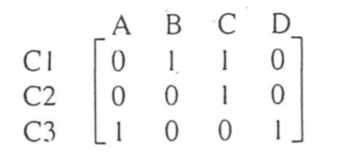
\includegraphics[scale=1]{images/acquiantace_table.png}\\
or in a graph form in which agents are nodes and skills are arches.\\
Finally there are two types of allocation depending on whenever the agents can delegate their request to other agents or not.

\paragraph{Direct Allocation}
In this mode an agent can have a task executed only by an agent that it knows directly \footnote{Similar to a single trader distribution system.}. If agent X wants task T to be executed it asks every agents it knows until someone respond positively.\\
We can address the issue of not finding any supplier by forcing allocation or using a centralized system which:
\begin{itemize}
\item Plays the role of maintenance and repair agent.

\item Will experience a low number of messages, since it is called only for extreme situations.
\item It can update the agents acquaintance tables in order to accelerate allocation process.
\end{itemize}

\paragraph{Allocation by delegation}
With this technique we can link together clients and suppliers which do not know each other directly. In this allocation mode a supplier that is asked to carry out a task can send it to another agent if it is not capable of doing it.\\
Parallel searching and diffusion algorithm \footnote{Like parallel breadth search.} can be used to propagate requests to all known agents. The are are some problems:
\begin{itemize}
\item Asking the same agent multiple time; can be fixed by marking the agent for that specific search \footnote{Problem arises to make skill search unique.}.
\item We want to make sure to search through the entire tree so we need acknowledges from every agent.
\end{itemize}  



Finally there are some imperfections:
\begin{itemize}
\item There is no optimization in term of agents skillfulness for a specific task.
\item Stop the search as soon as an agent has accepted the task
\item Unique task search key to avoid agent ignoring similar searches.
\end{itemize}


\paragraph{Reorganization of acquaintance network}

We can have environments in which the agents capabilities changes through time \footnote{Either agents enter/exit the system or their skills changes.} so we need to reorganize the acquaintance network. We can do it in two ways:
\begin{itemize}
\item When the agent A changes then it alert all the other agents known to A. Two problems:
	\begin{itemize}
	\item Need of bilateral contacts between acquaintance \footnote{If B is an acquaintance of A then A have to know its skills from B prospective.}.
	\item Parallelism synchronization between changes and new requests.
	\end{itemize}
\item When B asks A to execute a Task which is no longer capable of doing it can update its table. In this case the frequencies of changes becomes critical.
\end{itemize}


\subsection{Allocation by contract net (Distributed)}
The contract net is a task allocation mechanism based on a market-like protocol. The relationship between the \textit{manager} (client) and the \textit{bidders} (suppliers)  is channeled through a request for bids \footnote{Bids are offers.} submitted by the bidders.\\
It works as follows:
\begin{enumerate}
\item \textbf{Announcement}: the manager sends the description of the task to all those considered able to respond or to everyone.
\item \textbf{Bidding}: the bidders submit \textit{proposals} to the manager.
\item \textbf{Awarding}: the manager estimates the proposals and awards the contract to the best bidder.
\item \textbf{Expediting}: finally, the bidder awarded with the contract accepts or decline the task.
\end{enumerate}


\paragraph{Contract propagation language}
The request for bids includes: 
\begin{itemize}
\item Description of the task
\item Contract number
\item Definition of the qualities required for the task
\item Form of proposal
\item Expiry date
\end{itemize}
like in the following image:\\
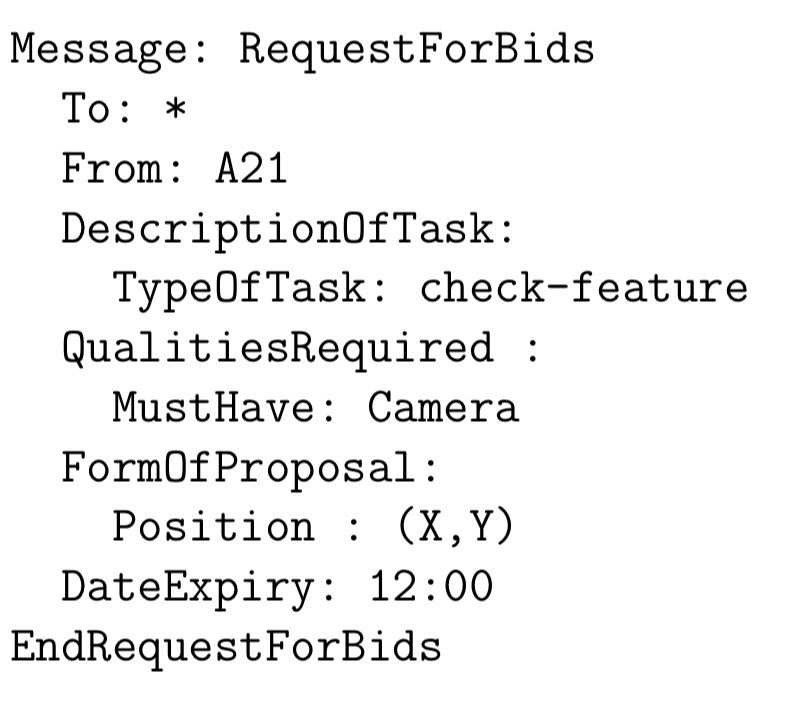
\includegraphics[scale=0.5]{images/contract_message.png}\\



\paragraph{Contacting bidders}
In general we can assume that all the agents in the network are accessible by any other, but obviously things are never this easy.\\
We can use algorithm for parallel search like the ones used for acquaintance net in the allocation by delegation part, so when the process is completed the manager can choose the best bid. The problem is that the agents does not know their neighbors' skills.\\
A solution may be a 	\textbf{token ring} where the manager hands the announce through a ring passing by every other agents.\\
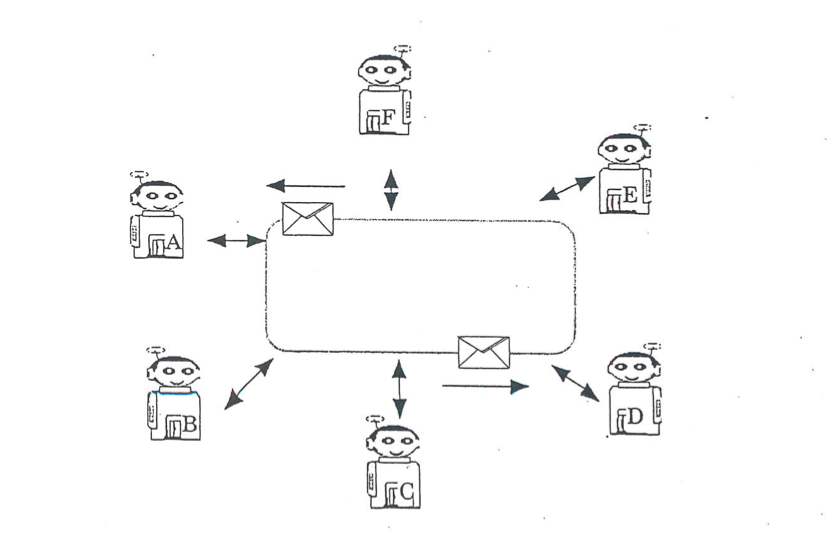
\includegraphics[scale=0.7]{images/contract_token.png}\\
This is not fast since the execution is sequential.


\paragraph{Limit date}
If the manager waits for the previous process to complete we have the following problems:
\begin{itemize}
\item Agents who are not interested in the task have to responds anyway, increasing both the number of messages and the time spent waiting. The solution is to not send message if not interested.
\item Agent that has experienced failure can block the system entirely. The solution is to add a deadline for receiving proposals.
\end{itemize}

\paragraph{Multiple manager and optimality}

There can be several manager issuing their request at the same time. Therefore we need to manage the concurrency for agents receiving multiple announcements since they can interfere with each other.\\
For Van Parunak the agents are ignorant in three ways:
\begin{itemize}
\item \textit{Temporal ignorance}: since bidders are aware of the request already received and not those arriving \footnote{An agent can accept a task which is not optimal for him, when another one could have been accepted some time later.}.
\item \textit{Spatial ignorance}: Manager does not know about other requests for bids in progress while bidders cannot know about other proposal. 
\item \textit{Ignorance of workloads}: bidders has no information of other agents' workloads.
\end{itemize}



\paragraph{Commitments, reservation and rejection of contracts}

Since we are working with concurrency we need to model the behavior in which new requests are receiven by bidders between the time they submit a proposal and the time they are rejected/awarded the contract. Should an agent which is waiting for the manager response take into account another proposal from another manager?

\begin{itemize}
\item If no, then the agent is working according to a \textbf{prudent} principle. Here the agent risk to end up without any work to do \footnote{For example given the bidder $A$ and two managers $X,Y$. $A$ has just submitted its proposal to $X$ ( which will be rejected) and it's waiting for a response, in the meantime the announce from $Y$ arrives (which will be accepted) and $A$ reject it a priori. Then $A$ ends up with no work to do. }. On the other hand the risk of overworking is minimized. This technique is useful when there \textit{aren't too many agents} submitting proposals.

\item If yes, then the agent is \textbf{brave} and it will not take into account the resource limit it has, and may end up with too much work to do. This method is more advantageous when there are a large number of agents in a competitive environment, where the probability of being awarded a contract is lower.

\item There is a middle way in which we associate two values to a task: the probability of obtaining the contract and the estimated profit and chose to reject/accept the task based on those.
\end{itemize}



\paragraph{Influence of sub-contractors}
Another possible implementation is the one where a bidder (B) who has been awarded with a contract decides to brake it down into \textit{sub-contract} \footnote{The same reasoning applies to this sub-contracts as the one for the sub-tasks. They must be as independent as possible to avoid redundant actions and cooperation.}. The bidder than becomes a manager itself and request bids for the sub-contract. There are multiple possibilities:
\begin{itemize}
\item \textbf{Early commitment} B makes up a team of sub-workers to complete the assignment \textit{after} submitting a proposal. The issue is when B cannot find any sub-workers for the sub-contract part, so it then tells its manager that he can no longer accept the contract and time is wasted.
\item \textbf{Late Commitment} B makes up a team of sub-workers to complete the assignment \textit{before} submitting a proposal. But we waste both time \footnote{If B is rejected then it must free its sub-workers} and can be stuck in deadlocks.
\item \textbf{Fixed agencies}: B is a boss of a small group of sub-workers which only accept assignments from B. This approach is less adaptive but more stable.
\end{itemize}

\paragraph{Pro/Cons of contract net}
\\
Pros:
\begin{itemize}
\item Allocation mechanism is simpler to implement.
\item Dynamic, no need for acquaintances management.
\item Based on bilateral agreement which can depend on multiple parameters \footnote{Such as agents' skills, workload, type of task/data...}.
\end{itemize}

Cons:
\begin{itemize}
\item Many messages $O(nm)$, good only for small societies.
\item Either the number of requests for bids is low or the data structures are complex for parallel implementation.
\item When the task can be broken down into sub-tasks the agents need a decision-making strategy for choosing commitment mechanism.
\end{itemize}


\paragraph{Proposal guided contract net}
We can invert the contract net protocol so that suppliers alert potential clients to their capacity. So the systems becomes proposal guided by the availability of the bidders.


\paragraph{Contract net vs acquaintance net}

\begin{itemize}
\item In acquaintances network agents' data \footnote{Such as skills, state ...} can be accessed directly by clients, while in contract net the agents have no priori knowledge of other agents, so they need to ask everyone. 
\item Acquaintance network lack dynamism, since any changes requires a network reorganization phase. 
\end{itemize}

We can try to merge this two approaches in the following ways:
\begin{itemize}
\item Using acquaintance for small tasks which are immediate and contract for big ones.
\item Acquaintance network can learn by using requests for bids every time it is necessary
\end{itemize}
Finally an acquaintance system can be seen as a cached memory of the contract net.




\newpage





\section{Auctions}
An auction can have the following proprieties:

\begin{itemize}
\item \textit{Guaranteed success}: agreement is certain to be reached.
\item \textit{Maximizing social welfare}: maximizes the sum of the utilities of negotiation participants.
\item \textit{Pareto efficiency}: a negotiation outcome is said to be Pareto efficient if there is no other outcome that will make at least one agent better off without making at least one other agents worse off.
\item \textit{Individual rationality}: where playing by the rules is in the best interest of negotiation participants.
\item \textit{Stability}: all agents have an incentive to behave in a particular way, e.g. Nash equilibrium.
\item \textit{Simplicity}: appropriate strategy for negotiation is \textit{obvious}.
\item \textit{Distribution}: there is no single point of failure and the communication between agents is minimized.

\end{itemize}

\paragraph{Mechanism Design}

\paragraph{Structure}
An action takes place between an agent known as \textbf{auctioneer} and a collection of \textbf{bidders}. The goal of the action is to allocate the \textit{good} to one of the bidders. While the auctioneer desires to maximize the price at which the good is allocated the bidders desires to minimize it.\\
There are many possible categories of auction based on:
\begin{itemize}
\item The \textit{value} of the good:

	\begin{itemize}
	\item \textbf{Common value}: when the good value is recognized the same by all the bidders, e.g. a dollar bill.
	\item \textbf{Private value}: the good has different value for each agent, e.g. grandpa's socks. 
	\item \textbf{Correlate value}: the value depends both on common and private value, e.g. buy a something with the intention of selling it later.
	\end{itemize}

\item The \textit{winner determination}, who gets the good?

	\begin{itemize}
	\item \textbf{First-price}: the agent that bid the most is allocated the good.
	\item \textbf{Second-price}: the agent that bid the highest is allocated the good, but pays the second-highest.
	\end{itemize}	 

\item The \textit{secrecy of bids}:

	\begin{itemize}
	\item \textbf{Open cry}: every agent know other agents' bids.
	\item \textbf{Sealed bid}: agents are not able to determine bids made by other agents.
	\end{itemize}
	
\item The \textit{auction procedure}:

	\begin{itemize}
	\item \textbf{One shot}: single round of bidding.
	\item \textbf{Ascending}: auctioneer starts from lowest price, bidders increase bids.
	\item \textbf{Descending}: auctioneer starts from high value and start decreasing it, the first bidder to accept the bid is the winner.
	\end{itemize}
	
\item Number of auctioneers/bidders:

	\begin{itemize}
	\item \textbf{Standard auction}: one seller, many buyers.
	\item \textbf{Reverse auction}: many sellers, one buyer.
	\item \textbf{Double auction}: many sellers, many buyers.
	\item \textbf{Combinatorial auctions}: buyers and sellers may have combinatorial valuations for bundles of goods.

	\end{itemize}

\end{itemize}


\paragraph{The winner curse}
When the auction is over, should the winner feel happy that they have obtained the good for less or equal to their private valuation? Or should they feel worried because no other agent valued the good as highly?\\
The situation in which the winner overvalues the good is known as the \textit{winner curse}.


\subsection{Types of auctions}


\paragraph{English Auction}
Is a \textit{first-price, open-cry, ascending} type of auction. 

\begin{itemize}
\item Protocol
\begin{enumerate}
\item Auctioneer starts by offering the good at a low price.
\item Bidders must offers higher prices.
\item The good is allocated to the agent that made the highest offer.
\end{enumerate}

\item Proprieties
\begin{itemize}
\item Generates competition between bidders (generates revenue for the seller when bidders are uncertain of their valuation).
\item  Dominant strategy: Bid slightly more than current bit, withdraw if bid reaches personal valuation of good.
\item Winner’s curse for common value goods.
\end{itemize}
\end{itemize}




\paragraph{Dutch auctions}
Is a \textit{open-cry, descending} auction. 

\begin{itemize}
\item Protocol
\begin{enumerate}
\item Auctioneer starts by offering the good at artificially high value.
\item  Auctioneer lowers offer price until some agent makes a bid equal to the current offer price.
\item The good is then allocated to the agent that made the offer.
\end{enumerate}

\item Proprieties
\begin{itemize}
\item Items are sold rapidly (can sell many lots within a single day).
\item  Intuitive strategy: wait for a little bit after your true valuation has been called and hope no one else gets in there before you (no general dominant strategy).
\item Winner’s curse possible.
\end{itemize}
\end{itemize}



\paragraph{First-price Sealed-bid auctions}
Is a \textit{one-shot, first-price, sealed-bid} auction. 

\begin{itemize}
\item Protocol
\begin{enumerate}
\item Within a single round bidders submit a sealed bid for the good.
\item  The good is allocated to the agent that made highest bid.
\item  Winner pays the price of highest bid.
\end{enumerate}

\item Proprieties
\begin{itemize}
\item Problem: the difference between the highest and second highest bid is “wasted money” (the winner could have offered less).
\item  Intuitive strategy: bid a little bit less than your true valuation (no general dominant strategy) \footnote{The more bidders the smaller the deviation should be.}.
\end{itemize}
\end{itemize}




\paragraph{Vickery auctions}
Is a \textit{second-price, sealed-bid, one-shot} auction. 

\begin{itemize}
\item Protocol
\begin{enumerate}
\item Within a single round bidders submit a sealed bid for the good
\item  The good is allocated to agent that made highest bid.
\item  Winner pays the price of the second highest bid.
\end{enumerate}

\item Proprieties
\begin{itemize}
\item Dominant strategy: bid your true valuation. If you bid more, you risk to pay too much. If you bid less, you lower your chances of winning while still having to pay the same price in case you win.
\item An antisocial behavior may occur in which a loosing agent \footnote{The agent must know that it is going to loose to another agent and the bid the other agent will make.} bid more than its true valuation to make opponents suffer (not “rational”).

\end{itemize}
\end{itemize}

\subsection{Lies and Collusion}
 
 There can be a collusion when groups of bidders cooperate in order to cheat. Bidders can agree beforehand to bid much lower than the public value so that when the good is obtained, the bidders can then obtain its true value and split the profits among themselves. All previous protocols are not collusion free, but they can prevent it by modifying the protocol so that bidders cannot identify each other.\\
There can be also be a lying auctioneer that places bogus bidders (shills) that artificially increase the price.

\subsection{Combinatorial Auctions}
Until now we talked about \textit{sequential} auctions where each good is sell sequentially and the determination of the winner is achieved by choosing the highest bid. A problem arises when the bidders have preferences over bundles \footnote{A bundle is a set of goods.}. In this case the bids will depend on \textit{speculation} on what others will bid in the future.\\

We can either use parallel auctions or combinatorial auctions.
In Combinatorial auctions the auctioneer puts several good on sale, each bidder must submit a bid for a bundle of goods. This is done in order to overcome the need for look-ahead \footnote{In which an agent will try to base its bid on the behavior of other. The results is that everyone will wait for someone to make the first move and a deadlock will occur.} and the inefficiencies that arises from the related uncertainties.\\
In this kind of setting there is an auctioneer that has a set of items $M=	\{1,2,...,m\}$ to sell, and there are $N$ buyers which submit a set of package bid $\mathbf{B}=\{B_1,B_2,...,B_n\}$, where $B_i=(S_i,p_i)$, where $S_i \subseteq M$ is a set of items and $p_i \ge 0$ is a price.\\
The \textbf{winner determination problem} is the problem of maximizing the sum of accepted bid prices:
\[max \sum_{j=1}^np_jx_j\] 
under the constrain that each item is allocated to at most one bid:
\[ \sum_{j|i\in S_j}x_j \le 1,\ \foralli \in \{1..m\},\ x_j \in \{0,1\}\]
and each agent receives at most one bundle:
\[\sum_{S \subseteq M} x_{S,i} \le 1,\ \forall i\in N\]
This problem is NP-complete and inapproximable.\\
We can use heuristic search to solve the problem representing the states with two possibilities.


\paragraph{Branch-on-items}
The question is \textit{What bid should this item be assigned to?}
So the state is represented by a set of items which have already been allocated and the branching is carried out by adding further items.\\
Each path on the search tree is a sequence of bids that do not share the same items with each other \footnote{Disjoint bids.} and it ends when there is no other bids to add.\\
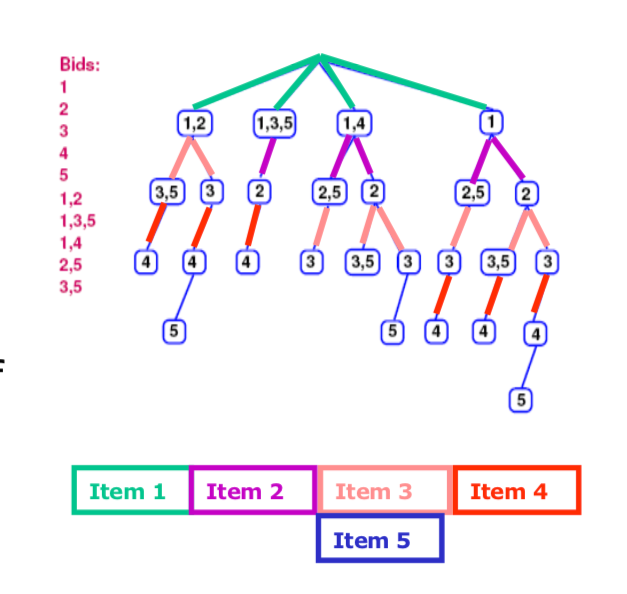
\includegraphics[scale=0.6]{images/branch_on_items.png}\\
As the search proceeds down a path a tally $g$ is kept of the sum of the prices; at every node the revenue $g$ form the current path is compared with the best $g-value$ found so far to determine if the current path is the best solution.\\
But the \textit{optimality} of the search my fall when there are some items with no bids or when the auctioneer makes better profit when keeping a bit. For example there is no bid for 1, there is a $5\$$ bid for 2 and a $3\$$ bid for [1,2]; the auctioneer makes better profit by selling \textit{only} 2. So he can make use of \textbf{dummy bids} of prices zero on those items with no 1-item bid.\\
Moreover we can reduce the brancing factor of a tree by remembering that the order of bids on a path does not matter. Finally the number of leaves can be no grater than $(\frac{n+n_{dummy}}{m})^m$, hence in the worst case the size of the tree is polynomial in the number of bids, but exponential in the number of items.


\paragraph{Branch-on-bids}
In this kind of search the question is \textit{should this bid be accepted or rejected?} \footnote{Since the possible answer is either yes or no, the tree is a \textit{binary tree}, so the branching factor is 2.}. The children in the search tree are the world where that bid is accepted (IN) and the world where the children is rejected (OUT).\\

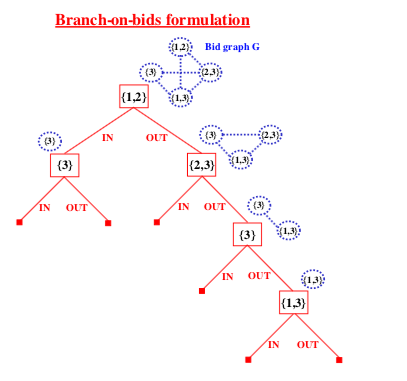
\includegraphics[scale=0.8]{images/branch_on_bid.png}\\

As you can see for the first bid (1,2), the children are the worlds in which it is accepted (left, IN) and rejected (right, OUT).\\
For this kind of search \textbf{no dummy bids} are needed, and the number of leaves is \textit{at most} $2^n$. Moreover this search is in line with the principle of \textit{least commitment} \footnote{Partial order planning.}, therefore we can refine the search control by ordering bids.


\paragraph{Heuristics}
Given $f(n)=g(n)+h(n)$ we have that:
\begin{itemize}
\item \textit{g(n)} is the revenue generated by bids that were accepted along the path.
\item \textit{h(n)} estimates for every remaining node in the current state, how much additional revenue can be expected.
\end{itemize}
Moreover we can prune large parts of state space by using \textbf{upper bounds} on how much the unallocated items can contribute; we simply sum over the unallocated items of the item's maximum contribution:
\[\sum_{i \in A}c(i),\ where\ c(i)=\max_{j|i\in S_j}\frac{p_j}{|S_j|}\]
Tighter bounds are obtained by recomputing $c(i)$ every time a bid is appended to the path.\\
Finally we can use the linear program relaxation of the remaining winner to determine the problem upper bound.

\subsection{Parallel Auctions}
Multiple items are open for auction simultaneously, bidders may place their bids during a certain time period, and the bids are publicly observable. Uncertainty and need for look-ahead are \textit{lowered} since their are partial signal to the bidder on what the others' bids will end up being.\\
Since each bidder would like to wait until the end to see what the going prices will be \footnote{In order to optimize its bids so as to maximize payoff given the final prices.}, there is a chance that no bidding would commence. As a patch to this problem, activity rules have been used.



\newpage


\section{Distributed Constrain Optimization Problem [DCOP]}
In DCOPs for MAS agents each agent negotiates locally with just a subset of other agents, called neighbors.
We work in a decentralized fashion for the usual reasons, such as \textit{robustness} \footnote{Avoid single point of failure.} and \textit{scalability} \footnote{Avoid excessive bandwidth allocation.}. On the other hand this approach can have some complications such as the need for \textit{distributed knowledge} ( since there is no centralize structure) \textit{information sharing} (i.e. the need of coordination) and \textit{complex systems} (which are difficult to design).\\
In this kind of problems each agent is considered \textit{benevolent}, that is the agents prefer to lose some optimization on its own valuation function in order to maximize the global function.

\paragraph{Constrain Networks}
A constrain network $\mathcal{N}$ is defined as a tuple $\langle X,D,C\rangle$ where:
\begin{itemize}
\item $X=\{x_1,x_2,..,x_n\}$ is a set of \textit{discrete} variables
\item $D=\{D_1,D_2,...,D_n\}$ is a set of variables domains for the corresponding variables, e.g. $x_i \in D_i$
\item  $C=\{C_1,C_2,...,C_m\}$ is a set of constrains which can be:

	\begin{itemize}
	\item \textbf{Hard}: when it defines a relationship $R_i$ between a subset of variables $S_i \subseteq X$, so that $R_i$ enumerates all the \textit{valid} assignment of $S_i$. This defines a \textit{Constraints Satisfaction Problem} CSP \footnote{Studied in the search part.} in which our aim is to \textit{find an assignment} for all the variables in the network that satisfy \textit{all the constraints}.
	\item \textbf{Soft}: when there is a function $F_i$ which maps every possible assignment of the subset $S_i$ to a real value. In this case we're facing a \textit{Constraints Optimization Problem} COP in which our aim is to find the \textit{best} solution rather than a valid one. So we need to define a global function $F(\overline{a})$ which is an aggregation of all the local functions $F_i(\overline{a}_i)$ in the problem, in which $\overline{a}_i$ are the restriction of $\overline{a}$ to $S_i$. 
	\end{itemize}
\end{itemize}
It is interesting to notice how a CSP can be turned into a COP by assigning a fixed cost to every violated constraint and search for an assignment that minimizes the sum of costs, this problem is known as \textbf{Max-CSP} problem.



\paragraph{Distributed Constraints Processing}

A DCOP can be represented as a constraint network $\mathcal{N}=\langle X,D,C\rangle$ plus a set of $k$  agents $A=\{A_1,A_2,...,A_k\}$, where each agent:
\begin{itemize}
\item  Can control \textit{just one} variable, for simplicity.
\item Is aware of the constraint that involves \textit{only} the variable that it controls.
\item Is considered a neighbor of another agents if there is \textit{at least one} constraint that depends on both. For this reason only neighbor agents can communicate with each other, which minimizes the amount of information that they must reveal to each other, thus preserving their privacy.
\end{itemize}


\paragraph{Benchmarking problems}
For example the \textit{graph coloring} problem which is a simple to formulate problem that can be easily modeled by a set of parameters \footnote{Like number of available colors, ratio between number of constraint and number of nodes.}. In this graph nodes are variables, the set of $k$ colors is the variable domain and the constraints are \textit{not-equal} that old between adjacent nodes. For example the following Figure is an instance of CSP on the graph coloring problem:\\
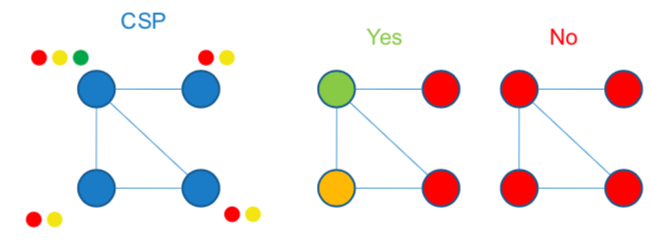
\includegraphics[scale=0.5]{images/graph_coloring.png}\\

\paragraph{Complete Algorithms}
We now focus on complete solutions techniques \footnote{Techniques which always find a solution.}, which are NP-Hard so the exhibit an exponentially increase in coordination overhead \footnote{Either size/number of messages or individual agent computation.} as the number of agents increases.\\
They can be divided in the following categories:
\begin{itemize}
\item \textit{Search based} algorithm, which can be divided into

	\begin{itemize}
	\item \textit{Synchronous} such as SyncBB, AND/OR search. Here the agents waits for messages from other agents before computing and sending messages themselves, which minimizes redundancy and uses only essential information.
	\item \textit{Asynchronous} such as ADOPT, NCBB and AB. Here agents performs computation and sends out messages without waiting, which makes use of parallel computation.
	\item \textit{optAOP} which is an algorithm that discovers pieces of the problem that are particularly hard to solve in a decentralized fashion, and centralizes them into sub problems that are delegated to mediators.
	\end{itemize}

\item \textit{Heuristic driven}  algorithm such as DSA,MGM, MAX-sum, which are \textit{not} guaranteed to find an optimal solution but have minimum coordination overhead
 agents.
 \item \textit{Approximate approaches}  such as Bounded max-sum, k-optimality, that both guarantees optimality and keeps a low coordination overhead.
\end{itemize}

\subsection{Dynamic Programming Optimization Protocol DPOP}
This algorithm is based on the distributed version of the \textit{Bucket Elimination} algorithm. It guarantees that the optimal solution can be found with a linear number of messages, and it has three phases:
\begin{enumerate}
\item Arrangement of variables into a DFS \footnote{Depth First Search.} tree \footnote{Can be build by token passing algorithm.}.
\item Propagation of \textit{Util} messages bottom-up along the DFS tree. In this part information are compiled to compute optimal values.
\item Propagation of Value message top-down the DFS tree, given the previous information the root chooses an optimal value and propagate the decision.
\end{enumerate}


\subsubsection{Pseudo-tree Ordering}
Given a graph G, a pseudo-tree is a rooted tree in which adjacent nodes\footnote{Variables which share some kind of constraint.} of G fall under the same branch \footnote{This leads to the conclusion that once a node is instantiated, its sub-trees are completely independent.}, i.e. belongs to the same path from the root to a leaf. It is easy to understand how a tree like this can be build using \textit{Depth First Search} (we will call the result DPS-tree and it will be a sub-class of the pseudo-tree) , since a path in it will be composed by only adjacent nodes. To build a pseudo-tree we first need an \textbf{ordering} of the nodes \footnote{Different ordering will lead to different pseudo-tree. Moreover finding the optimal ordering can be reduce to find the ordering which minimizes the separator $Sep_i$ size. } and the algorithm is the following:
\begin{enumerate}
\item Traverse the graph using a recursive procedure starting from the given \textit{ordering}.
\item Each time we reach a node $x_i$ form $x_j$ we mark $x_i$ as visited and we say that $x_j$ is the father of $x_i$, effectively creating a \textbf{tree edge}.
\item When $x_i$ has a visited neighbor $x_k$ that is not in the parent path we state that $x_k$ is a pseudo-parent of $x_i$, effectively creating a \textbf{back edge}.
\end{enumerate}

\paragraph{Example}
Given the graph $\mathcal{G}$ (Figure \ref{fig:graph_g}) where:
\[
\mathcal{G} = \begin{cases} C=\{X,D,C_{hard},C_{soft}\} \\
X=\{a,b,c,d,f,g\}\\
C_h=\{\}\\
C_s=\{F^a_b,F^b_d,F^a_b,F^a_c,F^b_c,F^b_f,F^c_f,F^f_g\}
 \end{cases}
\]

\begin{figure}[H]
\centering
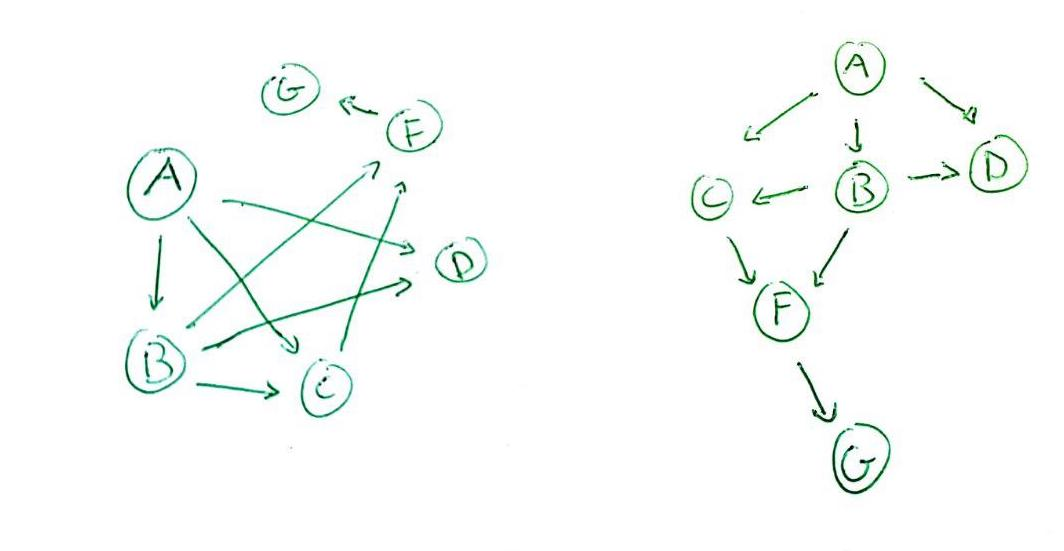
\includegraphics[scale=0.25]{images/dfs-tree_1.jpg}\\
\caption{Graph $\mathcal{G}$}
\label{fig:graph_g}
\end{figure}


And given the order $o: \{a,b,d,c,f,g\}$, the resulting DFS-tree $\mathcal{P}$ is:
\begin{itemize}
\item The Levels are: $L_0=\{a\},L_1=\{b\},L_2=\{c,d\},L_3=\{f\},L_4=\{g\}$
\item The Tree edges are: $\{F^a_b,F^b_d,F^b_c,F^c_f,F^f_g\}$
\item The Back edges are : $\{F^a_d,F^a_c,F^b_f\}$
\end{itemize}

As shown in Figure \ref{fig:dfs_p}

\begin{figure}[H]
\centering
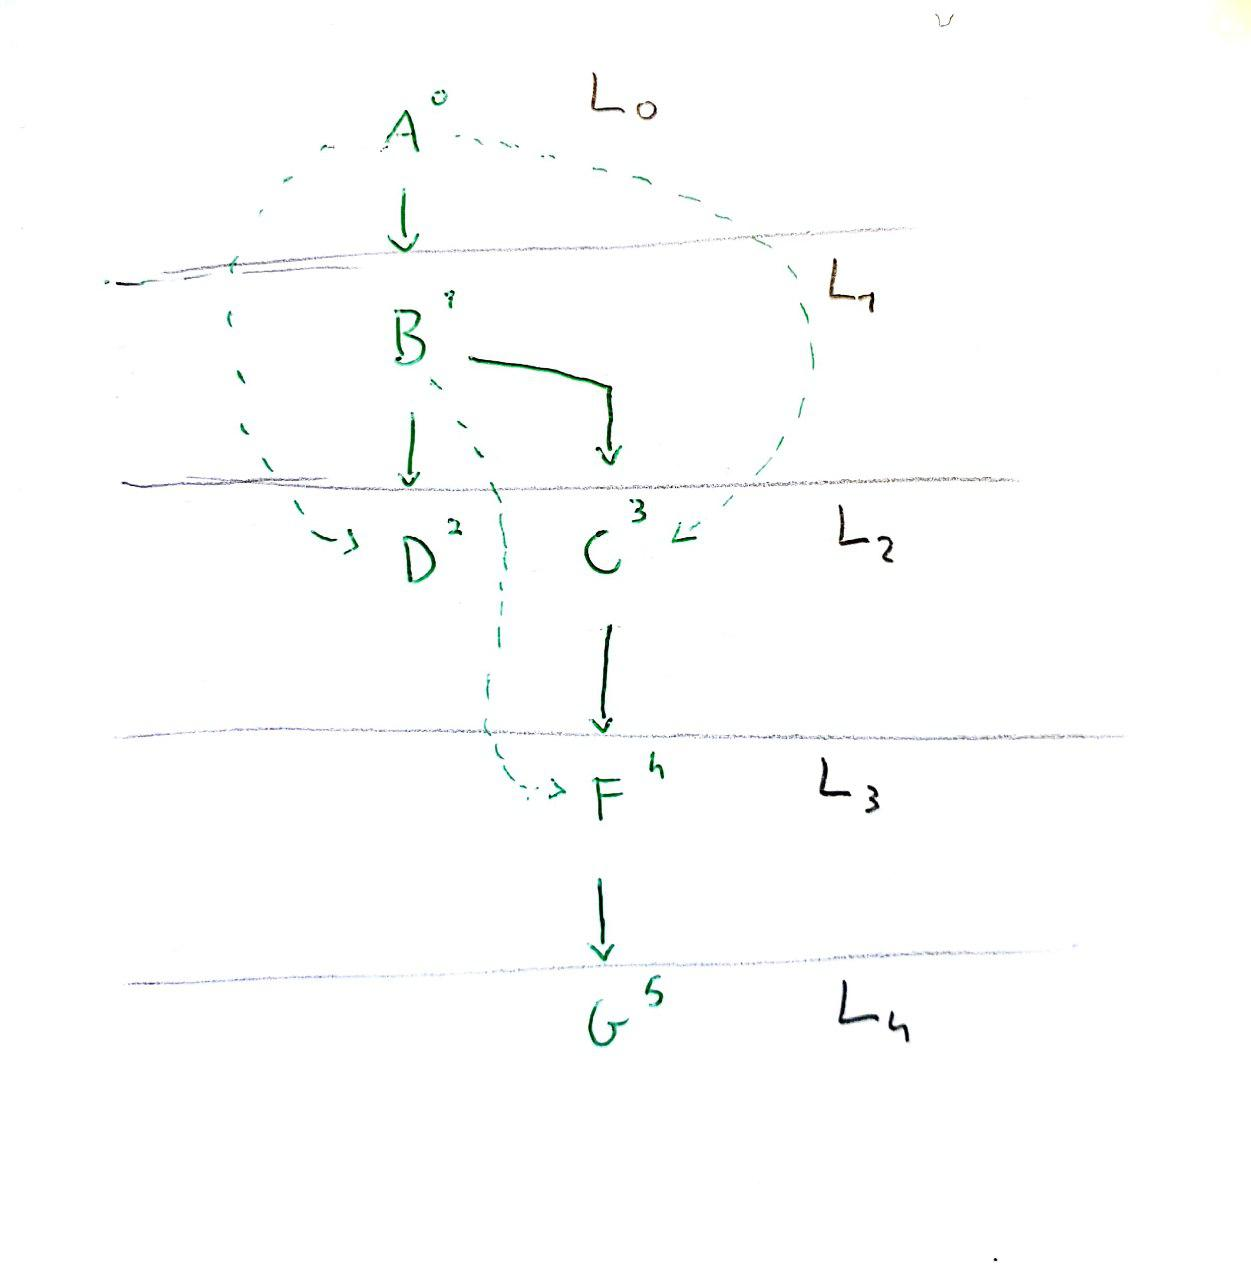
\includegraphics[scale=0.15]{images/dfs-tree_2.jpg}\\
\caption{DFS-tree $\mathcal{P}$}
\label{fig:dfs_p}
\end{figure}

\paragraph{Concepts}

Given two nodes $x_i,x_j$ we have that:
\begin{itemize}
\item If $x_j$ is an ancestor of $x_i$ through a \textit{tree edge}, then $x_i$ is a \textbf{children} $C$ of $x_j$, while the latter is the \textbf{parent} of $x_i$.
\item If $x_j$ is an ancestor of $x_i$ through a \textit{back edge}, then $x_i$ is a \textbf{pseudo-children} $C$ of $x_j$, while the latter is the \textbf{pseudo-parent} of $x_i$.
\item A \textbf{separator} of $x_i$, $Sep_i$ is a split (so a set of nodes) of the tree in two parts: one part is made up of all the ancestors which are connected with $x_i$ \footnote{Either through tree or back edges.}, the other one is made up of all the descendants of $x_i$. This set is called separator because it is precisely the set of agents that should be removed to completely separate the sub-tree rooted at $x_i$ from the rest of the network.
\item A \textbf{minimal separator} of $x_i$ are all the nodes that, if removed, completely disconnects the sub-tree rooted at $x_i$ from the rest of the problem.
\end{itemize}

\paragraph{Building DFS-tree in distributed system}
We can use the Token passing algorithm shown in Figure \ref{fig:token_pass}.

\begin{figure}[H]
\centering
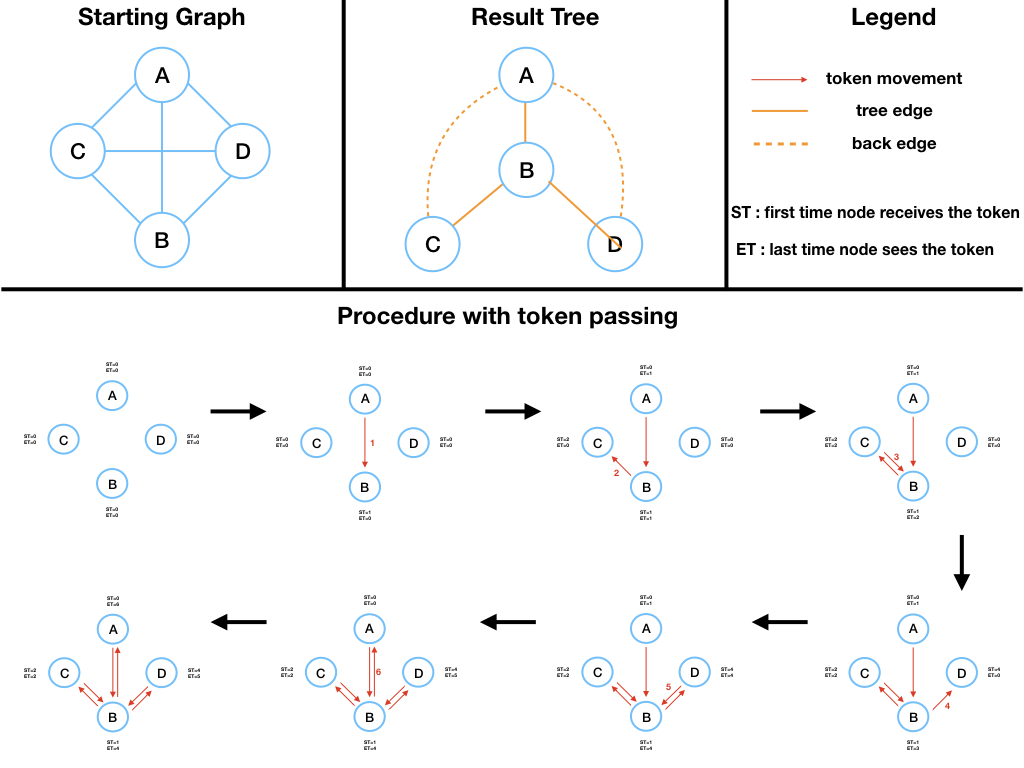
\includegraphics[scale=0.4]{images/token_passing.jpeg}
\caption{Token passing algorithm}
\label{fig:token_pass}
\end{figure}

\paragraph{Good heuristics}
Finally some good heuristic for this kind of problem are: Maximum Connected Node MCM and Maximum Cardinality Set for DFS.

\subsubsection{Util Propagation}
As before mentioned the Util propagation phase has a \textit{bottom-up approach} in which each node, starting from the leaves, computes a message \textit{for} its parent considering both: the messages received from its children and the constraints that agent is involved in.\\
The goal is to build a value function so that the root agent can make an optimal decision.\\
The formula for the Util message $U_{i\rightarrow j}$ that agent $A_i$ has to sent to its parent $A_j$ is:
\[U_{i\rightarrow j}(Sep_i)=\max_{x_i}\bigg(\bigoplus_{A_k \in C_i}U_{k\rightarrow i}\oplus \bigoplus_{A_p \in P_i \cup PP_i}F_{i,p}\bigg)\] s
Where:
\begin{enumerate}

\item $C_i$ is the set of children of agent $A_i$.
\item $P_i$ is the set of parent $A_i$.
\item $PP_i$ is the set of agents preceding $A_i$ that are connected thought a \textit{back edge}, i.e. its pseudo-parents.
\item $Set_i$ are the set of agents preceding $A_i$ that are connected either with $A_i$ or with one of its descendant. 
\item $A_p \in P_i \cup PP_i$ are all the agents $A_p$ which are either parents or pseudo-parents of agent $A_i$. 
\item The $\oplus$ operator is a join operator that sums up functions with different but overlapping scopes consistently, i.e. summing the values of the functions for assignments that agree on the shared variables.
\item $\bigoplus_{A_p \in P_i \cup PP_i}F_{i,p}$ is the joint summatory of the values driven by the soft constraints, either back or tree edges, for every parent, pseudo or non, of $A_i$.
\item While $A_k \in C_i$ are all the children of $A_i$
\item And $\bigoplus_{A_k \in C_i}U_{k\rightarrow i}$ is the joint summatory of all the messages coming from the children of $A_i$.
\item So that $\bigg(\bigoplus_{A_k \in C_i}U_{k\rightarrow i}\oplus \bigoplus_{A_p \in P_i \cup PP_i}F_{i,p}\bigg)$ is the joint sum of both the constraints carried from the children and the constraints $A_i$ has towards its parents. 
\item Finally the max operation is due to the necessity to take the value which maximizes the entire function.

\end{enumerate}

\paragraph{Example}
Given the DFS-tree in Figure \ref{fig:util_p}

\begin{figure}[H]
\centering
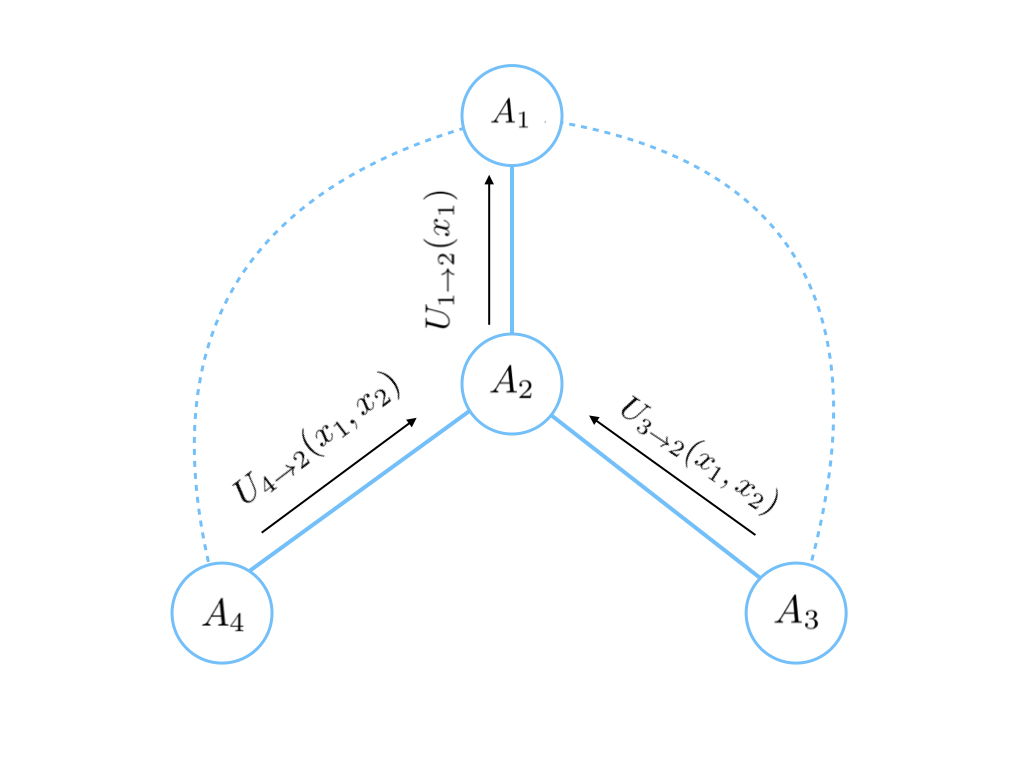
\includegraphics[scale=0.3]{images/util_p1.jpeg}
\caption{Util propagation}
\label{fig:util_p}
\end{figure}

We have that the values of the Util massages are the following:
\begin{itemize}
\item  $U_{3 \rightarrow 2}(x_1,x_2)=\max_{x_3}(F_{3,1}(x_3,x_1) \oplus F_{3,2}(x_3,x_2))$, where:
	\begin{itemize}
	\item  there is no contribution from $9$ since $A_3$ has no children.
	\item $ P_i \cup PP_i=\{A_2\} \cup \{A_1\}=\{A_2,A_1\}$ so that
	\item $F_{3,1}(x_3,x_1) \oplus F_{3,2}(x_3,x_2)$ is driven by $7$.
	\end{itemize}

\item  $U_{4 \rightarrow 2}(x_1,x_2)=\max_{x_4}(F_{4,1}(x_4,x_1) \oplus F_{4,2}(x_4,x_2))$, same as above

\item $\max_{x_2}(U_{3 \rightarrow 2}(x_1,x_2) \oplus U_{4 \rightarrow 2}(x_1,x_2) \oplus  F_{2,1}(x_2,x_1))$, where:

	\begin{itemize}
	\item $C_2=\lbrace A_3,A_2\rbrace$ so that
	\item $U_{3 \rightarrow 2}(x_1,x_2) \oplus U_{4 \rightarrow 2}(x_1,x_2)$ is generated by $9$,
	\item plus the part generated by $7$
	\end{itemize}


\end{itemize}



\paragraph{Message composition}
Given a graph coloring example, whit the graph in Figure \ref{fig:util_p}, in which we can have either black or white (0,1). We first consider the agent $A_3$ and we compute the Table \ref{tab:u32}. In this table we assign $-1$ if the is not respected (same color), $0$ otherwise.

\begin{table}[H]
\centering
\begin{tabular}{|l|l|l|l|l|l|}
\hline
x_1 & x_2 & x_3 &F_{3,1}  & F_{3,2} &F_{3,1}(x_3,x_1) \oplus F_{3,2}(x_3,x_2) \\ \hline
0 & 0 & 0 & -1 & -1 &-2  \\ \hline
\rowcolor{Gainsboro!60}
0 & 0 & 1 & 0 &  0& 0 \\ \hline
0 & 1 & 0 & -1 & 0 &-1  \\ \hline
0 & 1 & 1 & 0 &  -1& -1 \\ \hline
1 & 0 & 0 & 0 &  -1&-1  \\ \hline
1 & 0 & 1 & -1 &0  &-1  \\ \hline
\rowcolor{Gainsboro!60}
1 & 1 & 0 & 0 & 0 & 0 \\ \hline
1 & 1 & 1 & -1 & -1 & -2 \\ \hline
\end{tabular}
\caption{$U_{3 \rightarrow 2}(x_1,x_2)$}
\label{tab:u32}
\end{table}

\subsubsection{Value Propagation}
In this last phase the root agent $A_r$ computes $X_r^*$ \footnote{So actually deicing the value of its own node and leaving the rest to decide.} which is the argument that maximizes the sum of the messages received by all its children.\\
The generic agent $A_i$ computes:
\[x_i^*=argmax_{x_i}(\sum_{A_j \in C_i}U_{j\rightarrow i}(x_p^*)+\sum_{A_j \in P_i \cup PP_i}F_{i,j}(x_i,x_j^*))\]

The computation is very similar to the one in the Util propagation, in which we have two pieces of the equation. One representing the optimal values chosen for the current agent's parents, while the other one is the function specific of the agent. In particular:

\begin{itemize}
\item $x_p^*=\cup_{A_j\in P_i \cup PP_i}\lbrace x_j^*\rbrace$ is the set of optimal values of $A_i$'s pseudo/parents.

\item So that $\sum_{A_j \in C_i}U_{j\rightarrow i}(x_p^*)$  is the sum of all maximized values coming for the parent choices.

\item On the other hand $F_{i,j}(x_i,x_j^*)$ is the value of the agent $A_i$ function given the optimal values coming from its parent, and its own constraint.

\end{itemize}

After this computation, agent $A_i$ sends to its children $A_j$ the message:
\[V_{i\rightarrow j}=\lbrace x_i=x_i^*\rbrace\cup \bigcup_{X_k}\lbrace x_s=x_s^*\rbrace,\quad X_k=X_s \in Sep_i \cap Sep_j \]

in which:
\begin{itemize}
\item $\lbrace x_i=x_i^*\rbrace$ is the optimal value $A_i$ has chosen for itself.
\item $X_k$ are those agents who are pseudo/parents of both $A_i,A_j$ so that
\item $\bigcup_{X_k}\lbrace x_s=x_s^*\rbrace$ are tho optimal values this pseudo/parents have chosen for themselves.
\end{itemize}

Since the maximization formula is the same as the one in the Util propagation phase, we can store the values in a table, during the Util propagation phase, hence reducing the computation.

\newpage

\section{Swarm Robotics}
\label{sec:swarm_robotic}
Swarm robotics studies robotic systems composed of a multitude of interacting units. We can either gave homogeneous systems or few heterogeneous groups in which each unit is relatively simple and inexpensive.
Single units have limitations, either physical of functional, and may lack global information.

\subsection{Random Walks}
We need a basic search strategy that can be driven from the animal word based on the following \textit{missing assumption}:
\begin{itemize}
\item No individual knowledge
\item No memory of the path taken
\item No learning abilities 
\end{itemize} 
Although there must be some kind of information sharing between agents that leads to a trade-off between ability ti widely search the environment and ability to share information \footnote{This kind of problem may be tackled with special reverse behavior such as homing to a central place.}.\\
A random walk can be broken down to a sequence of alternate \textbf{straight motion} and \textbf{random turns}. There are two approaches for this kind of motion:

\subsubsection{Correlated Random Walks (CRW)}
In this kind of walks there is a positive correlation between consecutive movements, that is, walkers moves in similar directions with high probability. 

\paragraph{Turning angle}
The turning angle $\theta$ is chose from a wrapped Cauchy distribution with the following PDF \footnote{Probability density function.}:
\[f_w(\theta; p)=\frac{1}{2 \pi}\frac{1-p^2}{1+p^2-2pcos(\theta)},\quad 0<p<1\]
in which the parameter $p$ determine the skewness of the distribution as shown in Figure \ref{fig:crw_pdf}, the higher $p$ the less likely is the robot to deviate from its current direction. 


\begin{figure}[t]
\centering
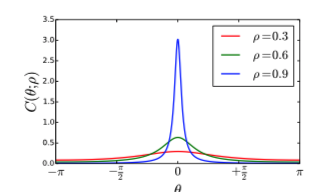
\includegraphics[scale=0.8]{images/random_walk.png}
\caption{PDF for CRW with different values of $p$}
\label{fig:crw_pdf}
\end{figure}

The correlation between movements is given by the $1+p^2-2pcos(\theta)$ parameter that, for higher thetas, decreases the output so that the orientation never changes too  much.
For $p=1$ we obtain a \textit{Dirac} distribution corresponding to a straight line motion, while for $p=0$ the distribution becomes uniform and provides no correlation between consecutive movements.

\paragraph{Straight motion}
For straight motion step, we define a distribution with finite second moment, so that the latter tends to a normal distribution according to central limit theorem.



\subsubsection{Lévy Walks (LW)}
This kind of random walk is characterize by several small displacement interleaved by long relocations. This provide an optimal search behavior for sparse targets since the long motion steps allow to search in different areas without frequently passing over sites that have been already visited.\\
The LW is characterized by a step-length distribution that follows a power law:
\[P_{\alpha}(t)\sim t^{-(\alpha+1)}\quad 0<\alpha \le 2\]
which can be defined in terms of Fourier transformation:
\[F(k)=e^{\-\beta|k|^{\alpha}}\]
for $\alpha=2$ the distribution becomes a Gaussian, while for $\alpha \rightarrow 0$ the random walk reduces to straight line paths.



\subsection{Aggregation}


Aggregation is a collective behavior that leads a group of agents to gather in some place. Therefore there is a transition from a homogeneous to a heterogeneous distribution of agents.\\
Depending on the presence of heterogeneities  \footnote{Heterogeneities (such as corners, shelters, humidity ecc...) can be exploited for aggregation.} in the environment we can have an easy problem. On the other hand, when no form of pre-existing heterogeneities can be found, the problem becomes more complex and an aggregation algorithm must be used.\\

There are two kind of aggregation algorithms:
\begin{itemize}
\item \textbf{Positive feedback} : in which agents emits signals that diffuses in space. The signal of neighboring agents sum up and becomes more attractive leading to the formation of large aggregates (Figure \ref{fig:positive_feed}).
\item \textbf{Social cues} : agents move randomly with certain probability to remain still for some time. The vicinity to other agents increases the probability of stopping and of remaining within the aggregate, eventually producing an aggregation process mediated by social influences (Figure \ref{fig:social_cues}). Aggregation is dependent on two main probabilities: the probability to enter an aggregate, which increases with the aggregate size, and the probability to leave an aggregate, which decreases accordingly.
\end{itemize}

\begin{figure}[H]
\centering
\begin{subfigure}
 \centering
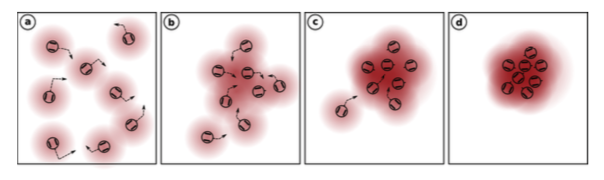
\includegraphics[scale=0.5]{images/positivie_feedback.png}
\caption{Positive feedback approach for swarm aggregation}
\label{fig:positive_feed}
\end{subfigure}%

\begin{subfigure}
\centering
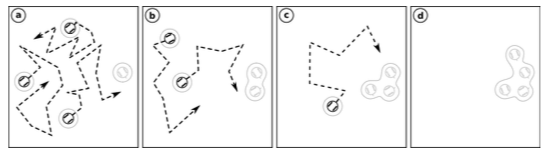
\includegraphics[scale=0.5]{images/social_cues.png}
\caption{Positive feedback approach for swarm aggregation}
\label{fig:social_cues}
\end{subfigure}%

\end{figure}

\subsection{Coordination}
In swarm robotics, ensuring coherence in space \footnote{That is display coordinated movement in order to maintain a consistent spatial structure.} is a fundamental propriety. We can have coordinated motion based on self-organization since we may have a non-uniform distribution of information, i.e.  having some agents that are more informed than the others on a preferred direction of motion.\\
We can have agents that are influenced solely by its nearest neighbor. Also, the movement of each agents is based on the same behavioral model, which includes also some inherent random fluctuation. We can use just three rules to model a fine behavior:
\begin{itemize}
\item Approach faraway individual.
\item Get away from agents that are too close.
\item Align with the neighbor direction.
\end{itemize}

\begin{figure}[t]
\centering
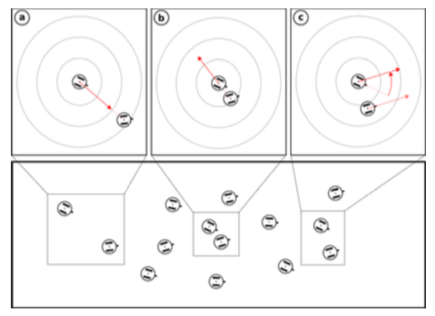
\includegraphics[scale=0.8]{images/coordination.png}
\caption{Coordination of swarm robots}
\label{fig:coordination}
\end{figure}

As shown in Figure \ref{fig:coordination}, when the nearest neighbor is within the closest region, the agent reacts by moving away. When the nearest neighbor is in the farthest region, the agent reacts by approaching. Otherwise, if the neighbor is within the intermediate region, the agent reacts by aligning.


\subsection{Collective Exploration}
Usually the swarm cannot completely perceive the environment, and the environment may also change during the operation of the robots; hence we need to lean on some common characteristic found in swarm robotic scenarios:
\begin{itemize}
\item A \textbf{central place} is a specific location where robots must come back regularly. A scenario that involves a central place requires a swarm able to either remember or keep track of that location.

\item If the environment is closed (\textbf{finite area}) and not too large, the swarm may use random motion to explore, with fair chances to rapidly locate resources (or even the central place). In an open environment, robots can get lost very quickly. In this type of environment, it is necessary to use behaviors that allow robots to stay together and maintain connectivity.

\item \textbf{Obstacles} are environmental elements that constrain the motion of the swarm. If the configuration of the obstacles is known in advance, the swarm can move in the environment following appropriate patterns. In most cases, however, obstacles are unexpected or might be dynamic and may prevent the swarm to explore parts of the environment.
\end{itemize}

\paragraph{CE in swarm robotics}
Animals also heavily rely on random motion to explore their environment . Usually the exploratory pattern is not fully random (that is, isotropic), because animals use all possible environmental cues at hand to guide themselves. Random motion can be biased towards a given direction, or it can be constrained in a specific area, for instance around a previously memorized location. For this reason the robot must have some kind of memory to avoid redundant search, either by means of localization techniques or by mapping the environment.\\
A collective motion aims at maintaining the cohesion between agents while moving through the environment. There are two possible implementations:
\begin{itemize}
\item The swarm can behave like a sort of physical mesh that covers part of the environment. This is called the \textbf{gas expansion} behavior where one robot keeps track of the central place while other agents spread as far as they can from each other while maintaining visual contact.
\item On the other hand swarms may form a \textbf{chain} whit one end that sticks to a central place and the other that moves freely through the environment \footnote{Allow to cover more area than the gas expansion behavior.}.
\end{itemize}


\subsection{Task allocation }
A \textit{response threshold model} assumes that each worker responds to a given stimulus when the stimulus intensity exceeds the worker's threshold. By allowing the threshold to vary in time with a reinforcement process \footnote{A threshold decreases when the corresponding task is performed, and increases when it is not performed.} we can have a more robust, general end long-time scaled model

\paragraph{Static model}
Consider:
\begin{itemize}
\item $m$ tasks that need to be performed
\item $\mathcal{N}$ workers, denoted by $i$ with
\item $\theta_{ij} (i=1,...,\mathcal{N};j=1,....,m$ response threshold, associated with task $j$.
\item $s_j$ is the intensity of task $j$.
\item $\mathcal{T}_{\theta_{ij}}(s_j)$ the probability for worker $i$ and task $j$, of "accepting the task".
\end{itemize}

In the fixed threshold model we have the probability of response equal to:
\[\mathcal{T}_{\theta_{ij}}(s_j)=\frac{s_j^2}{s_j^2+\theta^2_{ij}}\]

We have that:
\\
\begin{cases} \mathcal{T}_{\theta_{ij}}(s_j) \rightarrow 0 , & \mbox{if } s_j \ll \theta_{ij}\\
\mathcal{T}_{\theta_{ij}}(s_j) \rightarrow 1 , & \mbox{if } s_j \gg \theta_{ij}\\
\mathcal{T}_{\theta_{ij}}(s_j) =0.5 & \mbox{if } s_j = \theta_{ij}
\end{cases}
\\
That is lower $\theta_{ij}$ are more likely to respond to lower level of stimulus.

\paragraph{Dynamic model}

On the other hand we can have a time dependent threshold, given:
\begin{itemize}
\item $\zeta$: the coefficient that describes the learning
\item $\phi$: the coefficient that describes the forgetting
\end{itemize}
both assumed to be identical for all tasks.\\
An individual $i$ becomes \textit{more} sensitive \footnote{I.e. the agent has a better knowledge of task $j$, thus in the future it will be more likely to choose task $j$ for its familiarity.} by an amount $\zeta \delta t$ to a stimulus $s_j$ associated with the task $j$  when performing that task during the time period of duration $\delta t$:
\[\theta_{ij} = \theta_{ij} - \zeta\detla t\]


On the other hand, an individual $i$ becomes \textit{less} sensitive by an amount $\phi \delta t$ to a stimulus $s_j$ associated with the task $j$  when \textit{not} performing that task for a time period of duration $\delta t$:
\[\theta_{ij} = \theta_{ij} + \phi\detla t\]

Finally, given $x_{ij}$, i.e. the fraction of time spent by agent $i$ in performing taks $j$: the agent performs the task during $x_{ij}\delta t$ whitihn $\delta t$, and other tasks during $(1-x_{ij})\delta t$. The resulting cchange in $\theta_{ij}$ within $\delta t$ is given by:
\[\theta_{ij}= \theta_{ij}-x_{ij}\zeta\delta t+ (1-x_{ij})\phi\delta t \quad \theta_{ij} \in [\theta_{min},\theta_{max}]\]


\subsection{Collective decision making}
With swarm robotics it is frequent that agents have different opinion about the correct decision \footnote{Based on partial/incorrect information.}, hence a mean collective decision is needed.

\paragraph{Variants}
There are three kind of variants for decision making in swarm robotics:
\begin{itemize}
\item \textbf{Opinion propagation}: As soon as a group member has enough information about a situation to make up its mind, it propagates its opinion through the whole group. It allows for fast collective decision at the cost of robustness and accuracy, since messages can be corrupted.




\item \textbf{Opinion averaging}: All individuals constantly share their opinion with their neighbors and also adjust their own in consequence. This leads to a collective decision by the mean of an averaging function. It is more robust than the previous one but it works best when all individuals have roughly identical knowledge \footnote{When there are more individuals that have poor information, these are the one which will be chosen more often (oddly familiar).}


\item \textbf{Opinion amplification}:  All individuals start with an opinion, and may decide to change their opinion for another one. The switch to a new opinion happens with a probability calculated on the basis of the frequency of this opinion in the swarm. Practically, this means that if an opinion is more represented in the group, it has also more chances to be adopted by an individual, which is why the term amplification is used. Instead of adjusting opinions, agents adopt new opinion with some probability, which prevents the lack of good knowledge to result in poor decision making.
\end{itemize}

\paragraph{Decision making in swarm robotics}
Here, robots can share and merge their localization opinions when they meet, by means of local infrared communication. By doing so, robots manage better localization and improve their performance in the foraging task. Moreover, robots associate a confidence level to their estimates, which is used to decide how information is merged. If a robot advertises an opinion with a very high confidence, then the mechanism produces opinion propagation. Hence the two mechanisms of averaging and propagation are blended in a single behavior, and the balance between them is tuned by the user with a control parameter.


\end{document}
